\begin{figure}[htbp]
    \centering
    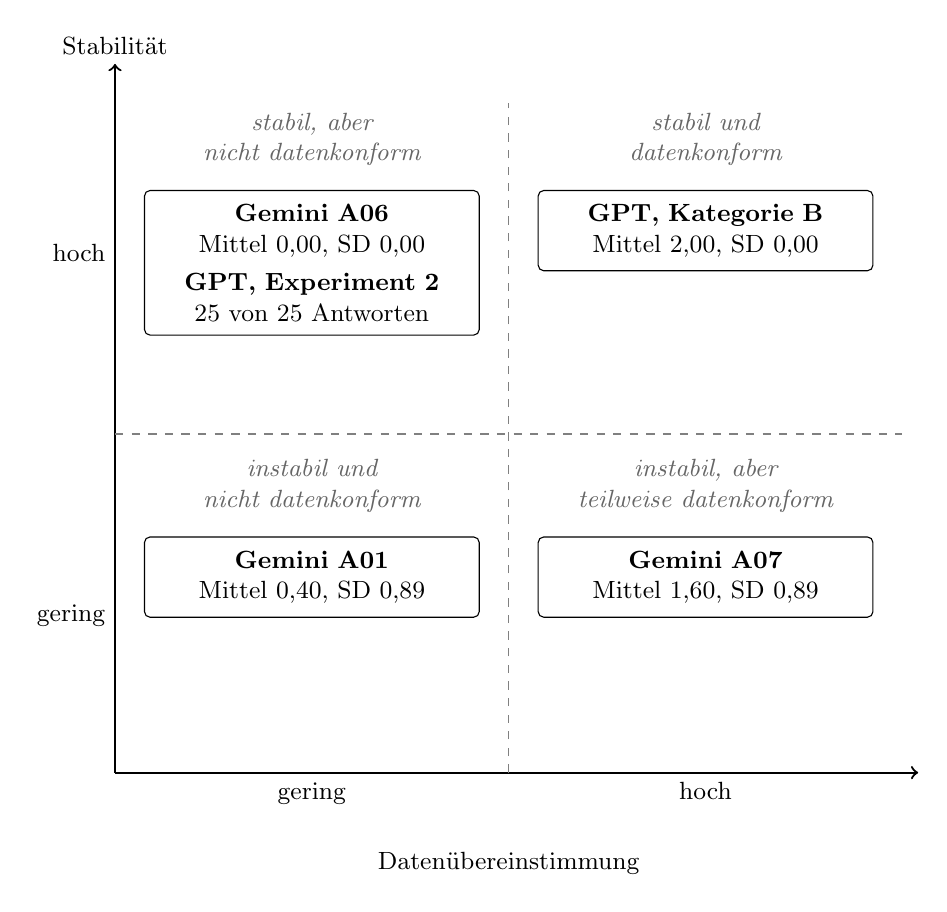
\begin{tikzpicture}[
        font=\small,
        beispiel/.style={
            draw,
            rounded corners=2pt,
            align=center,
            inner sep=5pt,
            text width=3.9cm,
            anchor=north
        },
        quadrant/.style={
            align=center,
            text=black!60,
            font=\small\itshape,
            anchor=north
        }
    ]
    % Achsen
    \draw[->, thick] (0,0) -- (10.2,0);
    \draw[->, thick] (0,0) -- (0,9.0);
    \node at (5.0,-1.15) {Datenübereinstimmung};
    \node[above] at (0,9.0) {Stabilität};
    % Trennlinien
    \draw[dashed, black!50] (5.0,0) -- (5.0,8.5);
    \draw[dashed, black!50] (0,4.3) -- (10.0,4.3);
    % Achsenbeschriftungen
    \node[below] at (2.5,0) {gering};
    \node[below] at (7.5,0) {hoch};
    \node[left] at (0,2.0) {gering};
    \node[left] at (0,6.6) {hoch};
    % Quadrantentitel, Oberkante fixiert
    \node[quadrant] at (2.5,8.5) {stabil, aber\\nicht datenkonform};
    \node[quadrant] at (7.5,8.5) {stabil und\\datenkonform};
    \node[quadrant] at (2.5,4.1) {instabil und\\nicht datenkonform};
    \node[quadrant] at (7.5,4.1) {instabil, aber\\teilweise datenkonform};
    % Beispiele, Oberkante fixiert, wachsen nach unten
    \node[beispiel] at (2.5,7.4)
        {\textbf{Gemini A06}\\
         Mittel 0,00, SD 0,00\\[3pt]
         \textbf{GPT, Experiment 2}\\
         25 von 25 Antworten};
    \node[beispiel] at (7.5,7.4)
        {\textbf{GPT, Kategorie B}\\
         Mittel 2,00, SD 0,00};
    \node[beispiel] at (2.5,3.0)
        {\textbf{Gemini A01}\\
         Mittel 0,40, SD 0,89};
    \node[beispiel] at (7.5,3.0)
        {\textbf{Gemini A07}\\
         Mittel 1,60, SD 0,89};
    \end{tikzpicture}
    \caption[Stabilität und Datenübereinstimmung]{
        Konzeptionelle Einordnung ausgewählter Ergebnisse entlang der
        Dimensionen Stabilität und Übereinstimmung mit der bereitgestellten
        Datengrundlage. Eine hohe Stabilität tritt sowohl bei zutreffenden
        als auch bei wiederholt abweichenden Antworten auf.
    }
    \label{fig:stabilitaet-datenuebereinstimmung}
\end{figure}